\chapter{Contact Force Control}

Since estimation algorithm has been created, force control of the arm for assembly tasks can be performed now. Instead of using F/T sensor to control the contact force, motor torques are used to control the contact force through the model. However, readings of F/T sensor are still captured to know the performance of the estimated model.

\section{Controller}
There are two controller that are used during this project to control the robot, they are force controller and position controller. Both controllers are PD controller with adjustable gain of P and D element.

\subsection{Force Controller}

force controller is a controller that use force as the input and feedback to drive the arm position. The figure below describes the block diagram of the force controller used. First a reference force is set, which after that the arm will move because of the difference between desired force and feedback force. The feedback force used will be calculated from the model prepared using motor torques and joint velocity. Hence, the algorithm will be used in this force controller architecture.

\begin{figure}[H]
    \centering
    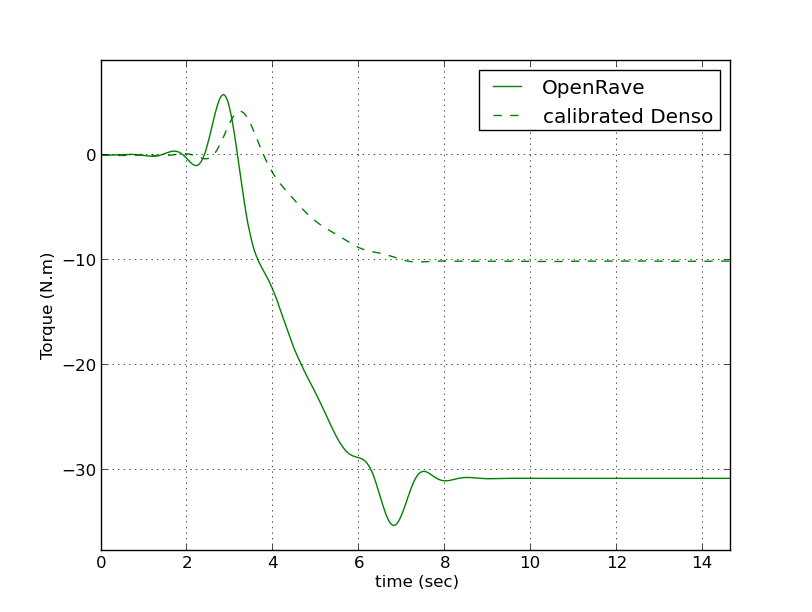
\includegraphics[width = 0.6\textwidth ]{high_tor_val}
    \caption{Force controller using motor torques and joint velocities}
    \label{fig: Force controller}
\end{figure}


\subsection{Position Controller}

Position controller is a controller that use position as the input and feedback to drive the arm position. It is more straightforward since it is position to position relation. It does not require force element in this controller and hence the algorithm created is not used in this function. See the figure below for the simple block diagram.

\begin{figure}[H]
    \centering
    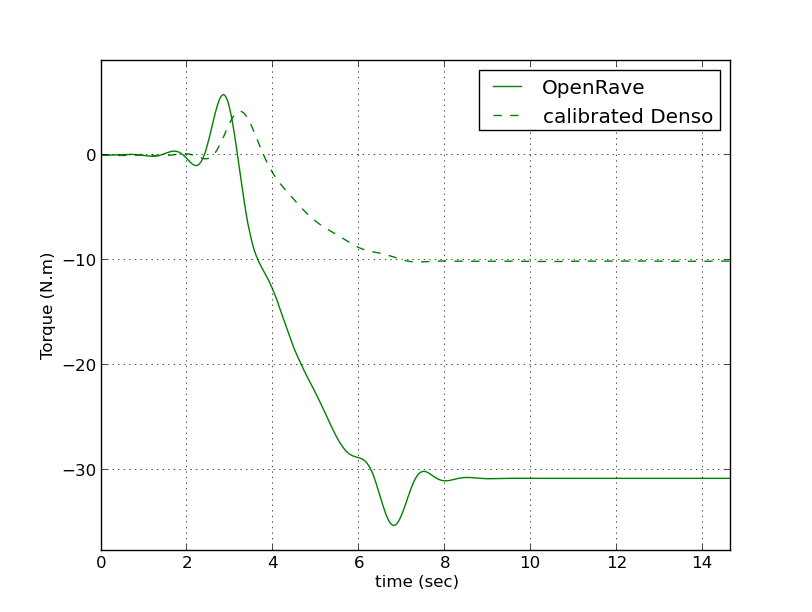
\includegraphics[width = 0.6\textwidth ]{high_tor_val}
    \caption{Position controller}
    \label{fig: Position controller}
\end{figure}


\section{Pin Insertion Task}

One assembly task that will be performed is the pin insertion task. Basically the robot has to search the hole in an object and then insert the pin into the hole. The general steps to perform this operation are:

1) Contact detection using position controller. The arm end-effector will move in z-axis based on position control. Force in z-axis ($F_{z}$) will be checked to determine when a contact with the plane is made. A contact is said to be detected once $F_{z}$ has exceed the threshold value, which in this task is set to be 20N.  

2) Hole detection using hybrid controller. After the robot has made a contact with the plane, the gripper holding the pin will move in the contact plane (x-y plane) using position control principle to search for the hole. The movement follows a spiral equation, where:

\begin{figure}[H]
    \centering
    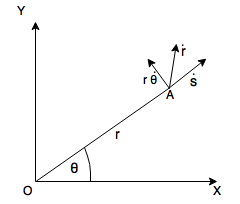
\includegraphics[width = 0.4\textwidth ]{spiral}
    \caption{Spiral movement vector}
\end{figure}

\begin{equation}
  \vec{\dot{r}} = \dot{s}\left(\left( cos\left(\omega t\right) - \omega t * sin\left(\omega t\right) \right)i + \left( sin\left(\omega t\right) + \omega t * cos\left(\omega t\right) \right)j\right)
\end{equation}

While it searches for the hole, the robot will also have to maintain the contact force $F_{z}$ with the plane, hence the manipulator will also need to move in z-axis. This movement is controlled by force controller. Thus, the gripper movement is controlled by both position and force controller and so it is called as hybrid controller. The contact force is maintained to be at 15N. To determine the hole existance, force in x and y-axis ($F_{x}, F_{y}$) are used as the indicator. It is set such that if the resultant force of ($F_{x}, F_{y}$) is greater than 60N for more than half second then the hole is detected.

3) Pin insertion using hybrid controller. When the hole has been detected, the final step is for the manipulator to insert the pin into the hole. To do this force controller is used to position the arm in x-y plane so that the pin will stay inside the hole while position controller is used to insert the pin in z-axis. The force controller in x-y plane is set to stay at 15N for each axis. The pin is said to be successfully inserted if $F_{z}$ is bigger than 80N.


All these steps will be executed using motor torques as the replacement of the F/T sensor. However since data from F/T sensor are also recorded, the force control performance using motor torques can be compared with the F/T sensor.

After several tuning to the PD gain in the controller, the manipulator was able to successfully insert the pin. The performance during the operation will be discussed in the next subsections.

\subsection{Contact Detection}

As what has been described in section \ref{algorithm}, the robot needs to move into the precontact position as close as possible to the plane of interest. In this case, the reference point is taken when the robot is not moving yet. This is to check whether it friction parameters that has been identified is good enough to compensate for the friction. After referencing to this point, the arm moves slowly approaching to the contact area. The force is then estimated using motor torques and joint velocities. 

The result of using the motor torques to estimate the end-effector force can be examined in \fref{fig:contact detection}. Results from ATI F/T sensor are also attached in the figure for comparison. The results show that the force estimation in x and y are not really reliable. This may indicate that the friction model identified might be off from the true friction such that it still produce some offset for the force estimation. Other reasons for this might be because the results of neglecting some important parameters such as torques for dynamic motion and deadzone problem during the identification.

\begin{figure}[h]
  \begin{subfigure}[t]{0.5\textwidth}
    \centering
    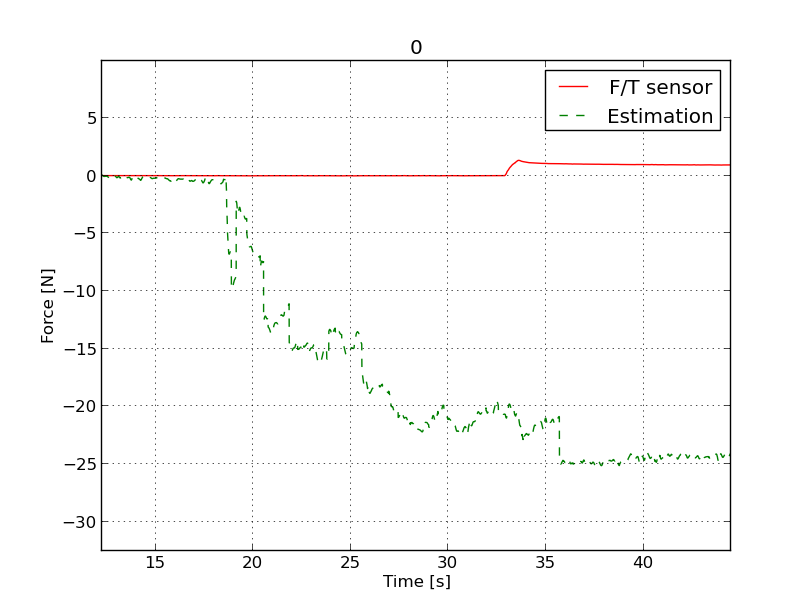
\includegraphics[width = \textwidth ]{contact_detection_x} 
    \caption{Force -x}
  \end{subfigure}
  \begin{subfigure}[t]{0.5\textwidth}
    \centering
    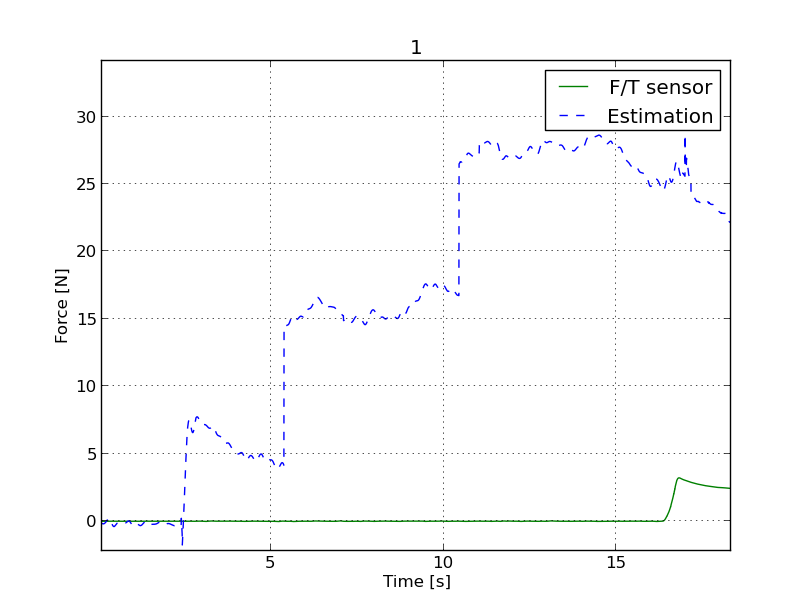
\includegraphics[width = \textwidth ]{contact_detection_y}
    \caption{Force -y}
  \end{subfigure}
  \begin{subfigure}[t]{0.5\textwidth}
    \centering
    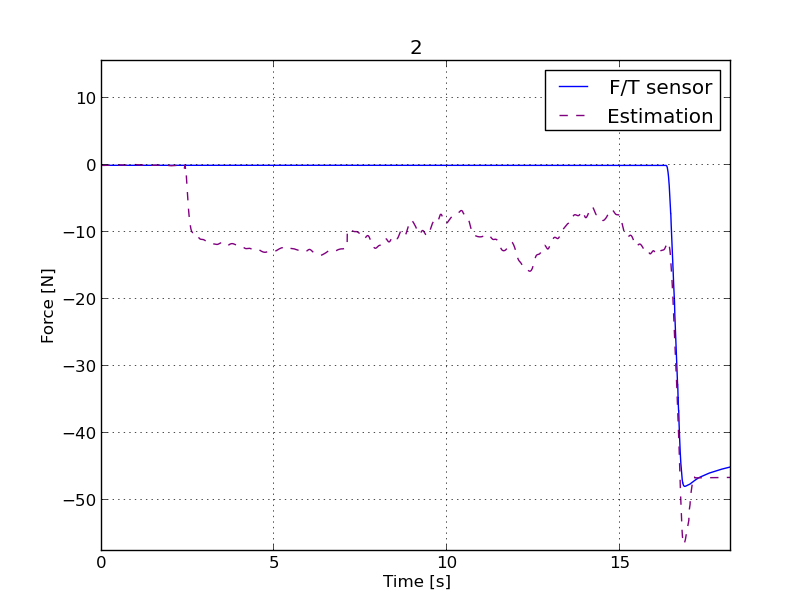
\includegraphics[width = \textwidth ]{contact_detection_z}
    \caption{Force -z}
  \end{subfigure}  
  \caption{Force estimation in contact detection. (- - : estimated output, -- : F/T sensor output)}
  \label{fig:contact detection}
\end{figure}

In contrast, force estimation in z direction is much better than the other two axis. While the average of $F_{z}$ is not zero, it is still below the threshold. There is also a clear difference in $F_{z}$ value where it easily exceed the threshold when a contact is happening. Furthermore, The value is comparable with the F/T sensor data when there is a contact. Hence, it is seen that using the estimation algorithm, contact detection can still be performed without F/T sensor.

One hypotesis on why it gives reasonable result only for z-axis is because the end-effector is only moving in z-axis and thus, it gives good estimation only on this axis. The implication of this is that the estimation in the other direction will be not good enough as what is seen in \fref{fig:contact detection}. This point will be investigated further in the next discussions. 

\subsection{Force Control in Hyrbrid Controller for Hole Detection}

The force data for all axis during this process are shown in \fref{fig:force control hole}. The continuous line represent the results from F/T sensor while discontinuous line is the computed force without F/T sensor.

\begin{figure}[h]
  \begin{subfigure}[t]{0.5\textwidth}
    \centering
    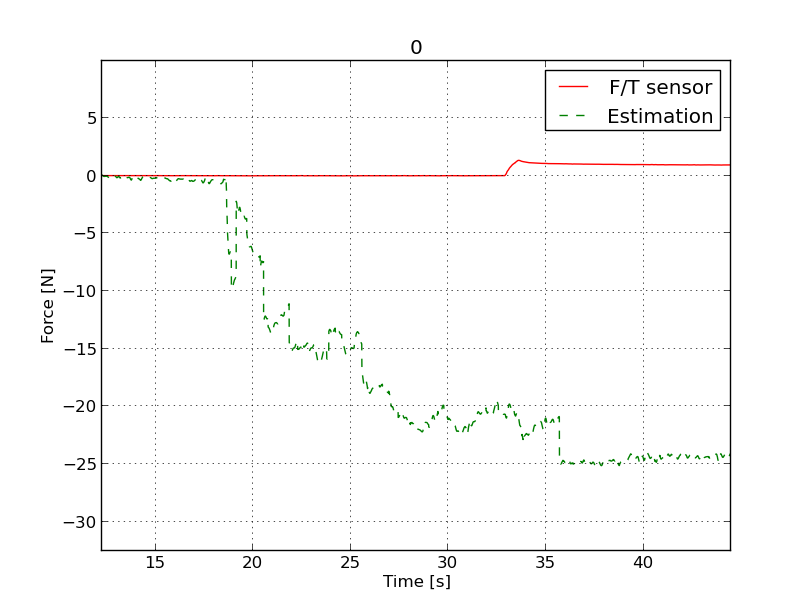
\includegraphics[width = \textwidth ]{contact_detection_x} 
    \caption{Force -x}
  \end{subfigure}
  \begin{subfigure}[t]{0.5\textwidth}
    \centering
    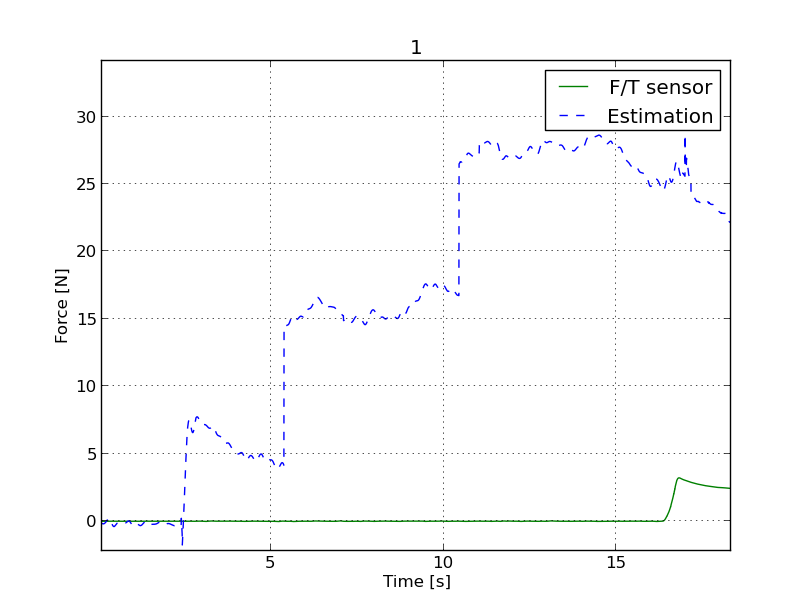
\includegraphics[width = \textwidth ]{contact_detection_y}
    \caption{Force -y}
  \end{subfigure}
  \begin{subfigure}[t]{0.5\textwidth}
    \centering
    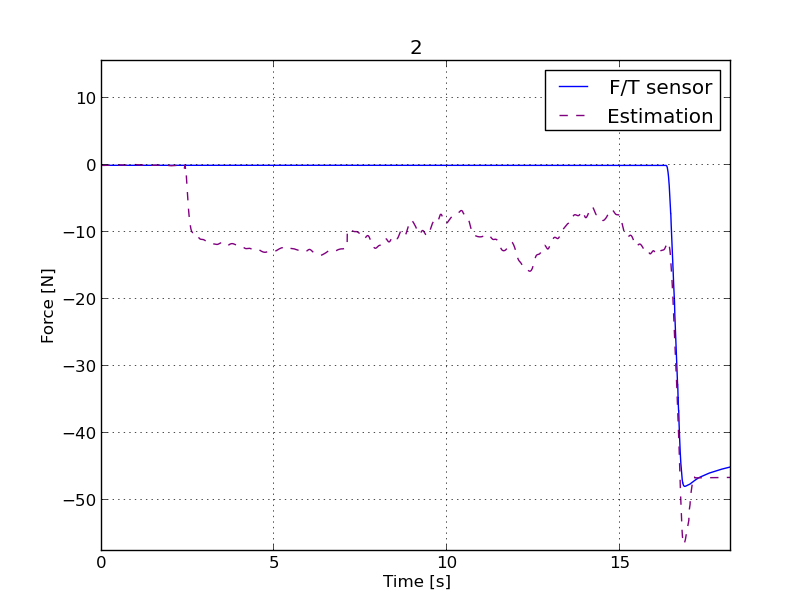
\includegraphics[width = \textwidth ]{contact_detection_z}
    \caption{Force -z}
  \end{subfigure}  
  \caption{Force for all axis during hole detection. (- - : estimated output, -- : F/T sensor output)}
  \label{fig:force control hole}
\end{figure}

During the early stage of the searching, the force control in z-axis is unstable. This is due to the fast change in the joint velocities during the early spiral movement where the circle line is near zero. However after several seconds the force become more stable and oscillate in around reference value which is 15 N. 

Comparison with the F/T sensor shows that the result from the model tend to underestimate the force and hence, leading to the actual force greater than computed. The F/T sensor have an average value of ... N (thus ....$%$ error) during the force control. While this performance is not wanted, this is better than overestimating the force. Since in this case it will be guaranted that the actual contact will have to happen first before the robot know about the contact. Thus, in this case the contact with the surface plane is still occuring during the hole searching.  

\subsection{Force Control in Hyrbrid Controller for Pin Insertion}

The force data for all axis during this final step are shown in \fref{fig:force control pin}. The continuous line represent the results from F/T sensor while discontinuous line is the computed force without F/T sensor.

\begin{figure}[h]
  \begin{subfigure}[t]{0.5\textwidth}
    \centering
    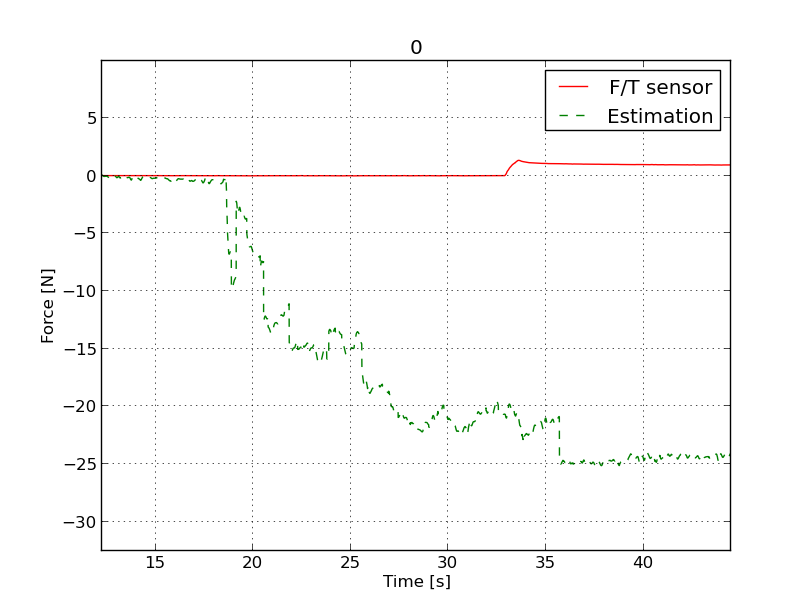
\includegraphics[width = \textwidth ]{contact_detection_x} 
    \caption{Force -x}
  \end{subfigure}
  \begin{subfigure}[t]{0.5\textwidth}
    \centering
    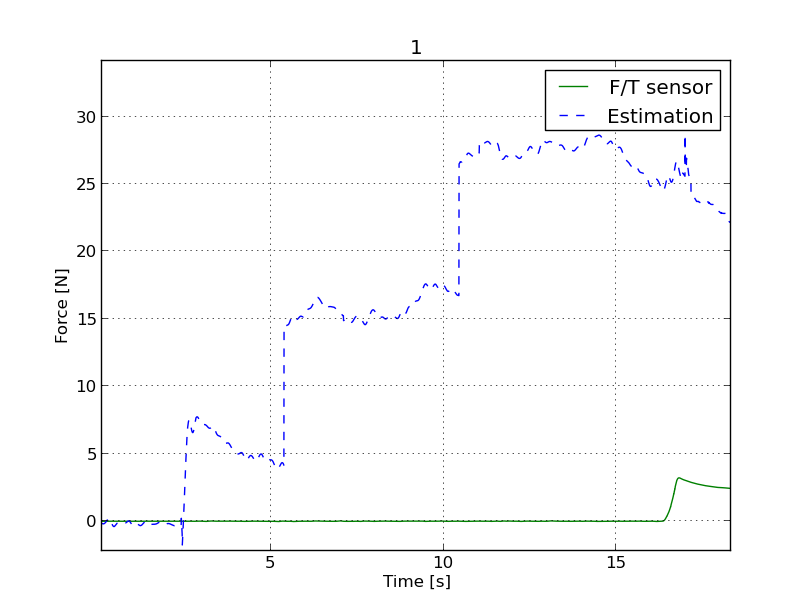
\includegraphics[width = \textwidth ]{contact_detection_y}
    \caption{Force -y}
  \end{subfigure}
  \begin{subfigure}[t]{0.5\textwidth}
    \centering
    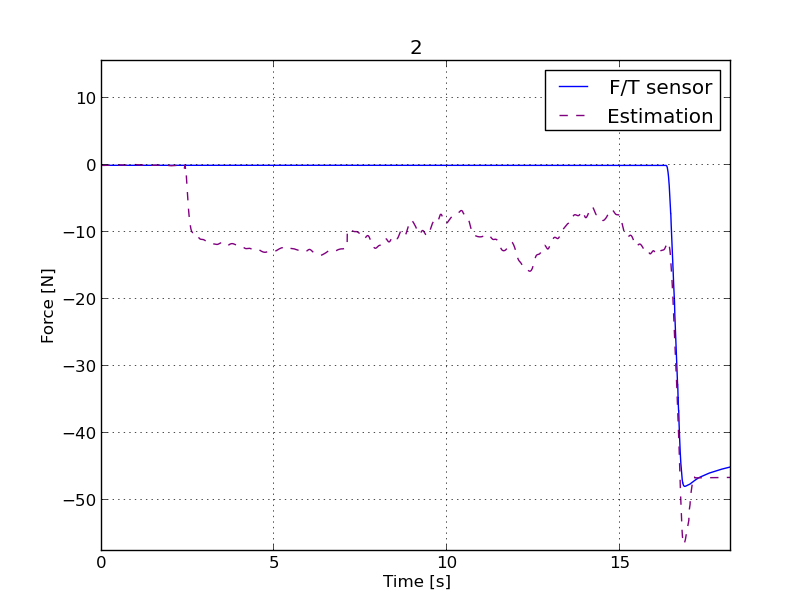
\includegraphics[width = \textwidth ]{contact_detection_z}
    \caption{Force -z}
  \end{subfigure}  
  \caption{Force for all axis during pin insertion. (- - : estimated output, -- : F/T sensor output)}
  \label{fig:force control pin}
\end{figure}

In this process two identical force controller is set to control each x and y position. Apart from the first few seconds where $F_y$ tend to be overestimated, the force controllers give similiar performances with the previous force controller, that is the algorithm tend to underestimate the contact force between pin and the object. Different behaviour is also found in the $F_z$ when the pin has been inserted. A positive force is observed from F/T sensor while the model estimated the force to be below -80N. 


In overall, while the estimated force is still not accurate according to F/T sensor, it gives the same pattern with the F/T sensor with underestimated value. Moreover it has been shown that it can be used as the force controller to control the contact force due to the underestimate behaviour of the model. 

